\documentclass{beamer}

\usepackage[utf8]{inputenc}
\usepackage[brazil]{babel}
\usepackage{graphicx,hyperref,icmc,url}
\usepackage{subcaption}
\usepackage{multirow}
\usepackage{tikz}
\newcommand{\destaq}[1]{\textcolor{purple}{\textbf{#1}}}

% The title of the presentation:
%  - first a short version which is visible at the bottom of each slide;
%  - second the full title shown on the title slide;
\title[Reconstrução de curvas por características robustas extraídas de imagens]{Reconstrução de curvas por meio de características robustas extraídas de imagens}

% Optional: a subtitle to be displayed on the title slide
\subtitle{Atividades realizadas}

% The author(s) of the presentation:
%  - again first a short version to be displayed at the bottom;
%  - next the full list of authors, which may include contact information;
\author[André Luís Mendes Fakhoury]{
    \Large{André Luís Mendes Fakhoury} \\ \medskip
    \small{\href{mailto:andrefakhoury@usp.br}{\nolinkurl{andrefakhoury@usp.br}}} \\ \bigskip
    \small{Orientador: João do Espirito Santo Batista Neto}
}

% \\ \bigskip
    % \large{}

% The institute:
%  - to start the name of the university as displayed on the top of each slide
%    this can be adjusted such that you can also create a Dutch version
%  - next the institute information as displayed on the title slide
\institute[ICMC/USP]{
    Vinculado ao projeto: ``Mapeamento de características robustas entre diferentes domínios e espaços $\mathbb{R}^2$ e $\mathbb{R}^3$''\\ \medskip
    Instituto de Ciências Matemáticas e de Computação -- ICMC \\
    Universidade de São Paulo - USP
}

% Add a date and possibly the name of the event to the slides
%  - again first a short version to be shown at the bottom of each slide
%  - second the full date and event name for the title slide
\date[4/5/2021]{\footnotesize{4 de maio de 2021}}

\AtBeginSection[]
{
    \begin{frame}<beamer>{Sumário}
        \tableofcontents[currentsection]
    \end{frame}
}

\begin{document}
    
    \begin{frame}[plain]
        \titlepage
    \end{frame}
    
    \begin{frame}
      \frametitle{Sumário}
      \tableofcontents
    \end{frame}
    
%%%%%%%%%%%%%%%%%%%%%%%%%%%%%%%%%%%%%%%%%%%%%%%%%%%%%%%%%%%%%%%%

\section{Resumo do projeto}
\begin{frame}
\frametitle{Resumo do projeto}
\framesubtitle{Introdução}

\begin{figure}[hbt]
	\begin{center}
		\caption{Diagrama de bloco das etapas de desenvolvimento}
		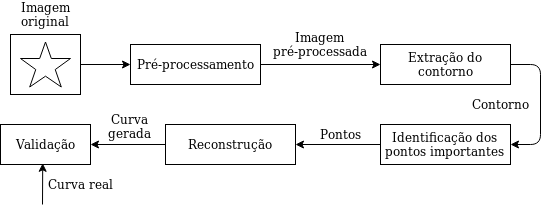
\includegraphics[width=1\textwidth]{img/diagrama.png}
	\end{center}
\end{figure}

\end{frame}


\begin{frame}
	\frametitle{Resumo do projeto}
	\framesubtitle{Exemplo (simples)}
	
	\begin{figure}[ht!]
		\centering
		\begin{subfigure}[b]{0.19\textwidth}
			\centering
			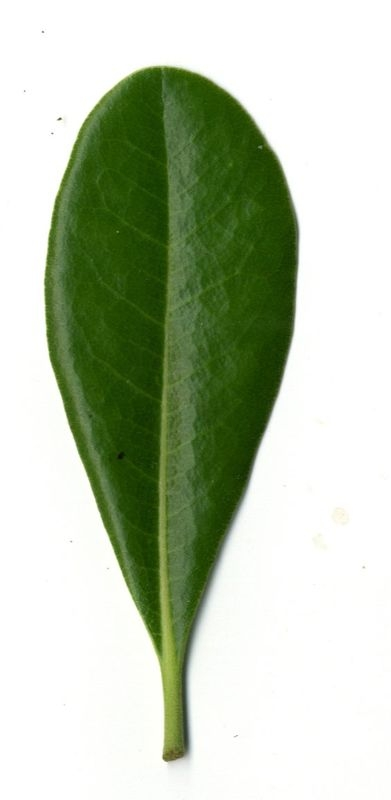
\includegraphics[width=\textwidth]{img/original.jpg}
		\end{subfigure}
		\begin{subfigure}[b]{0.19\textwidth}
			\centering
			
\includegraphics[width=\textwidth]{img/preprocess.jpg}
		\end{subfigure}
		\begin{subfigure}[b]{0.19\textwidth}
			\centering
			
\includegraphics[width=\textwidth]{img/contour.jpg}
		\end{subfigure}
		\begin{subfigure}[b]{0.19\textwidth}
			\centering
			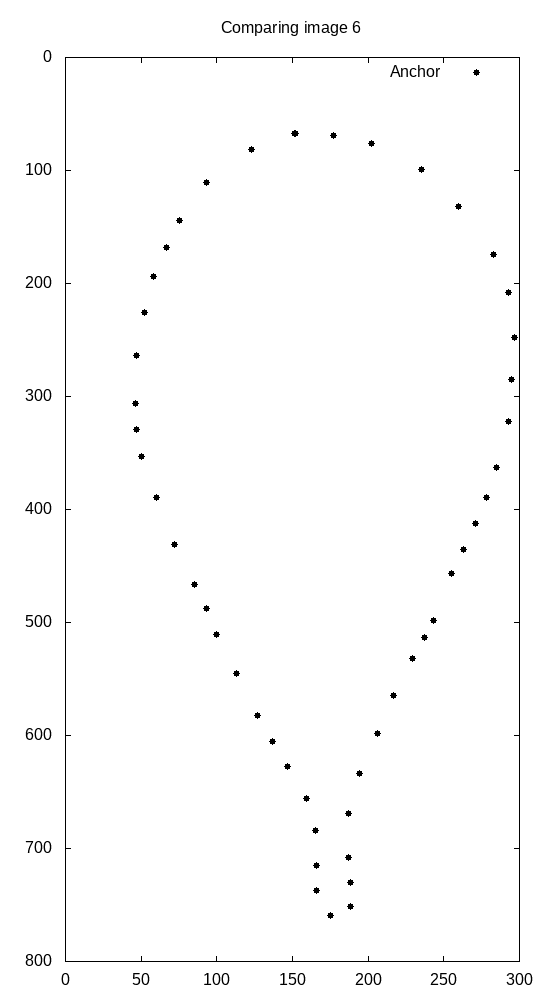
\includegraphics[width=\textwidth]{img/points.png}
		\end{subfigure}
		\begin{subfigure}[b]{0.19\textwidth}
			\centering
			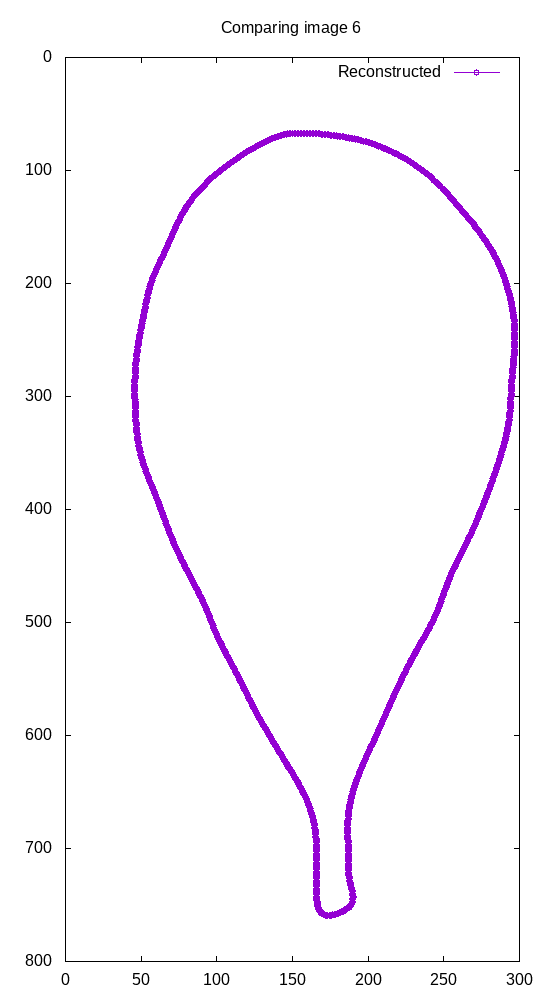
\includegraphics[width=\textwidth]{img/reconstructed.png}
		\end{subfigure}
		\label{fig:editedmesh}
	\end{figure}
	
\end{frame}




\section{Atividades realizadas}
\begin{frame}
	\frametitle{Atividades realizadas}
	\framesubtitle{Durante as ``férias''}
	
	\begin{itemize}
		\item Passagem de \destaq{MatLab} para \destaq{C++};
		\item \textit{Pipeline} para testar várias imagens de uma vez;
		\item Teste com imagens de banco de dados com folhas \cite{imageclef2011}, comparando escolha dos pontos âncora de maneira aleatória, linear ou por curvatura.
	\end{itemize}
	
\end{frame}


\begin{frame}
	\frametitle{Atividades realizadas}
	\framesubtitle{Exemplos de resultados (figura 6, 65 pontos)}
	
	\begin{figure}[ht!]
		\centering
		\begin{subfigure}[t]{0.24\textwidth}
			\centering
			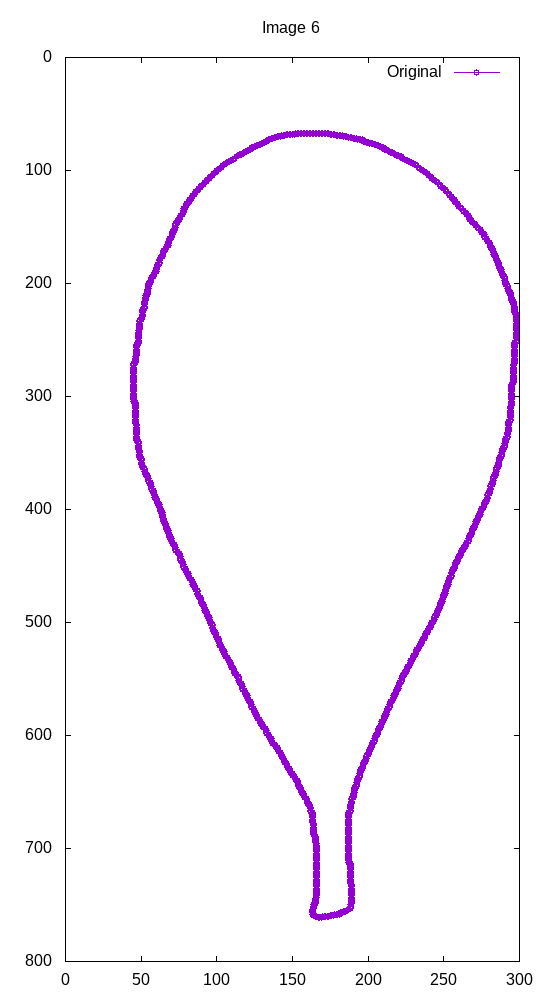
\includegraphics[width=\textwidth]{img/rec/6ori.png}
			\caption{Curva original}
		\end{subfigure}
		\begin{subfigure}[t]{0.24\textwidth}
			\centering
			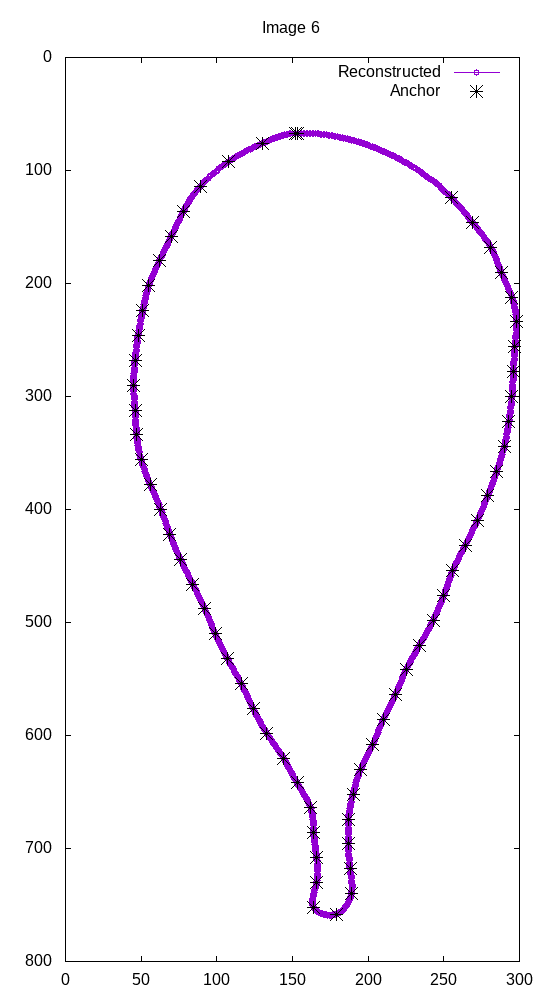
\includegraphics[width=\textwidth]{img/rec/6lin(781).png}
			\caption{Linearmente espaçados (781)}
		\end{subfigure}
		\begin{subfigure}[t]{0.24\textwidth}
			\centering
			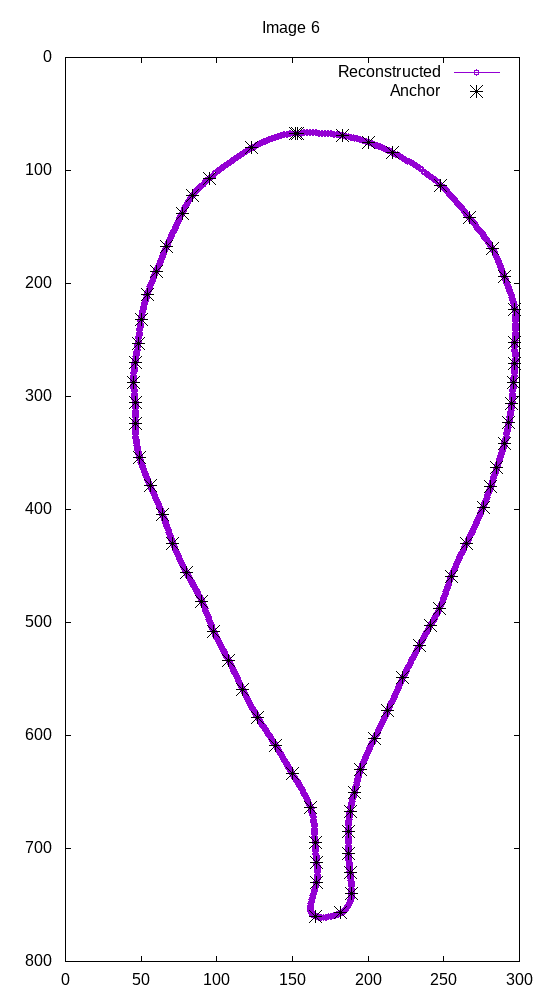
\includegraphics[width=\textwidth]{img/rec/6cur(663).png}
			\caption{Curvatura (663)}
		\end{subfigure}
		\begin{subfigure}[t]{0.24\textwidth}
			\centering
			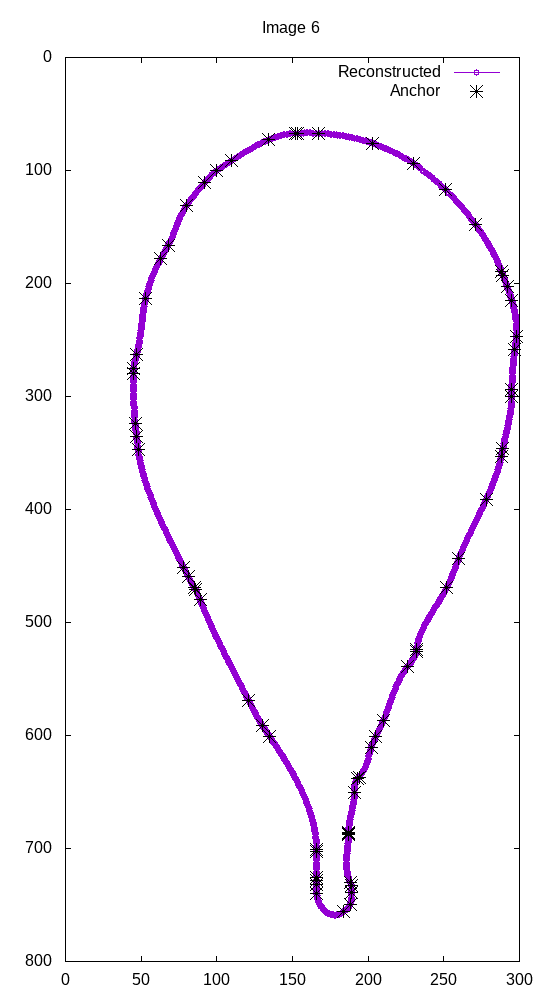
\includegraphics[width=\textwidth]{img/rec/6rng(1139).png}
			\caption{Aleatórios (1139)}
		\end{subfigure}
		\label{fig:rec6}
	\end{figure}
\end{frame}

\begin{frame}
	\frametitle{Atividades realizadas}
	\framesubtitle{Exemplos de resultados (figura 11, 65 pontos)}
	
	\begin{figure}[ht!]
		\centering
		\begin{subfigure}[t]{0.24\textwidth}
			\centering
			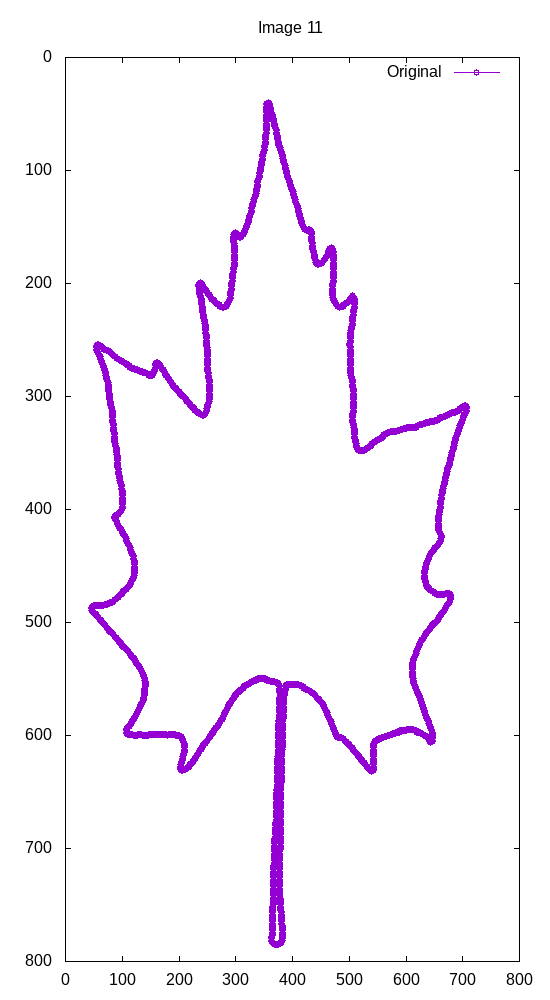
\includegraphics[width=\textwidth]{img/rec/11ori.png}
			\caption{Curva original}
		\end{subfigure}
		\begin{subfigure}[t]{0.24\textwidth}
			\centering
			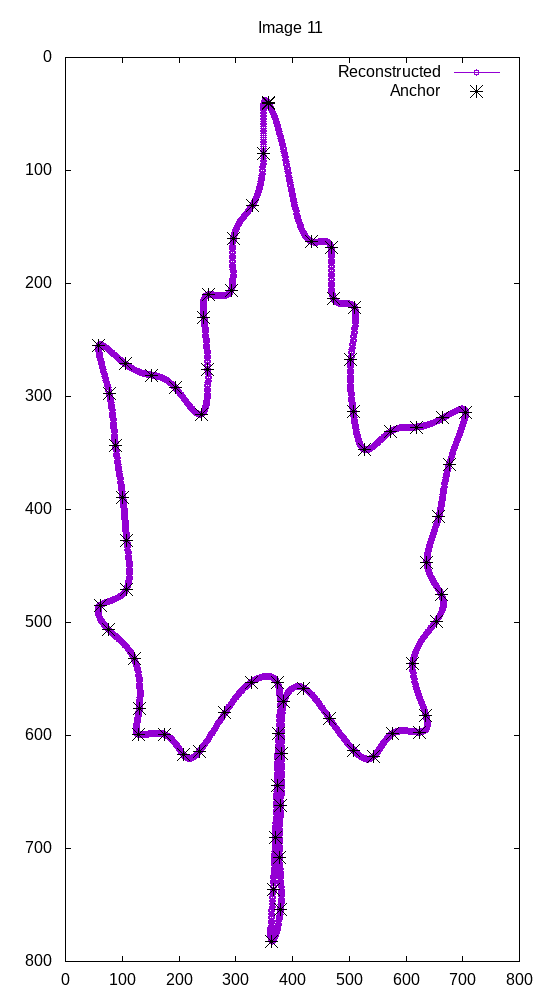
\includegraphics[width=\textwidth]{img/rec/11lin(11594).png}
			\caption{Linearmente espaçados (11594)}
		\end{subfigure}
		\begin{subfigure}[t]{0.24\textwidth}
			\centering
			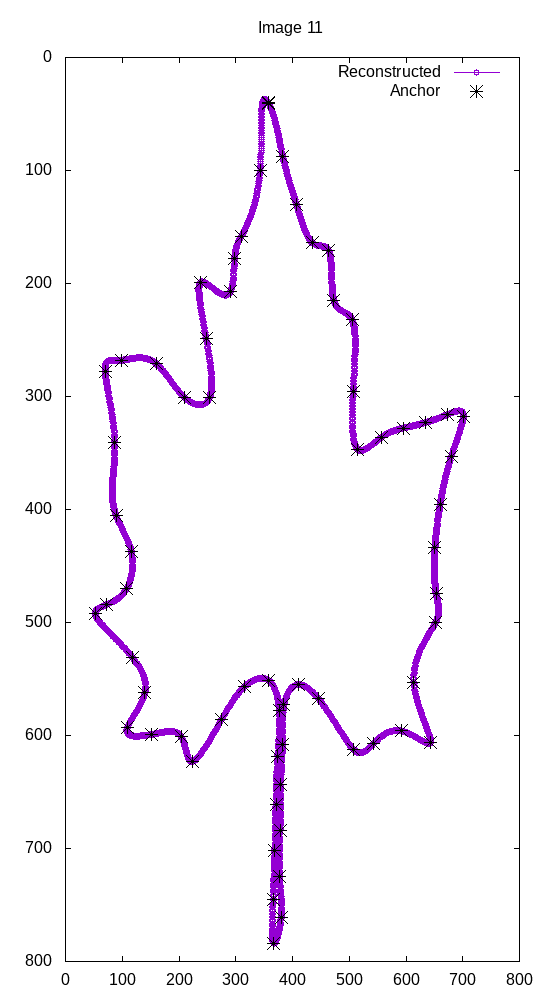
\includegraphics[width=\textwidth]{img/rec/11cur(13512).png}
			\caption{Curvatura (13512)}
		\end{subfigure}
		\begin{subfigure}[t]{0.24\textwidth}
			\centering
			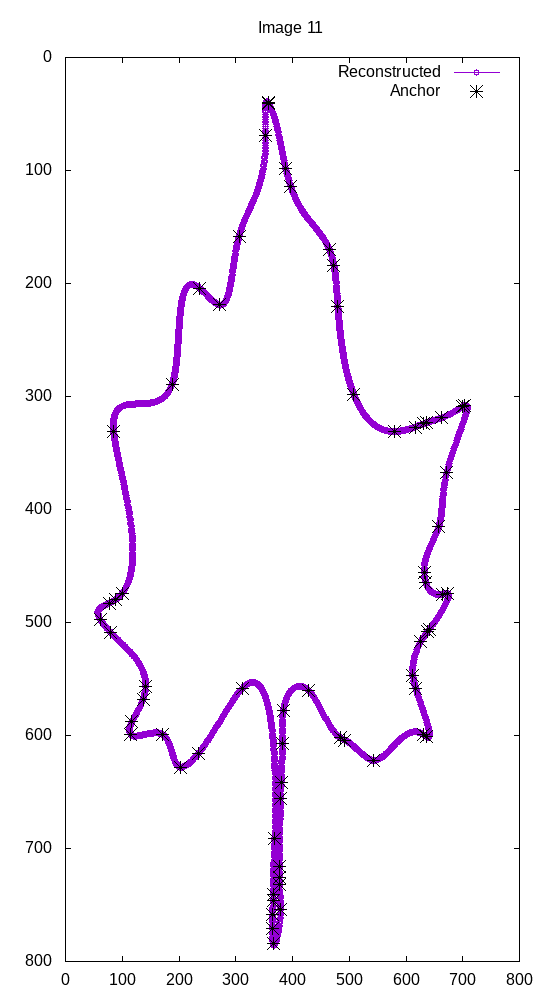
\includegraphics[width=\textwidth]{img/rec/11rng(32340).png}
			\caption{Aleatórios (32340)}
		\end{subfigure}
		\label{fig:rec6}
	\end{figure}
\end{frame}

\begin{frame}
	\frametitle{Atividades realizadas}
	\framesubtitle{Exemplos de resultados (figura 64, 65 pontos)}
	
	\begin{figure}[ht!]
		\centering
		\begin{subfigure}[t]{0.24\textwidth}
			\centering
			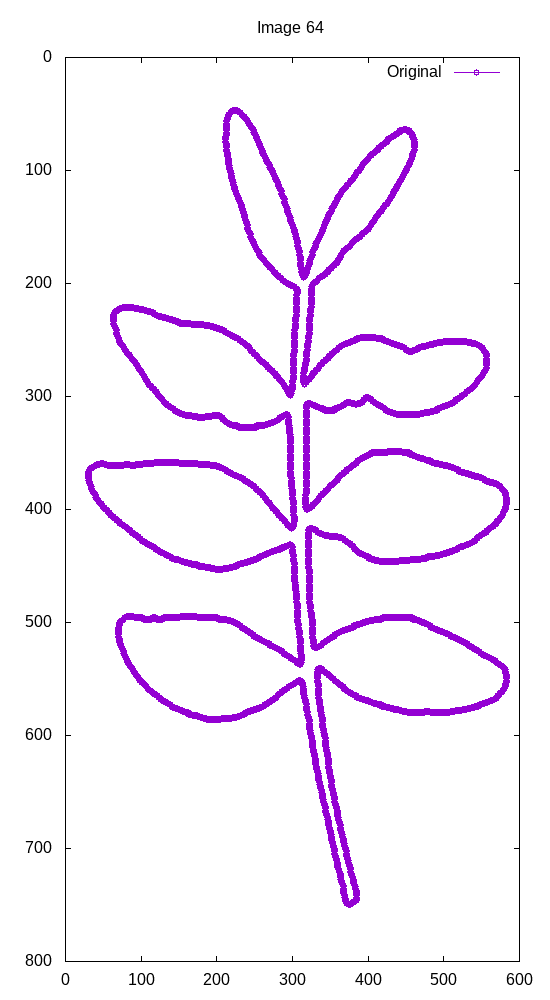
\includegraphics[width=\textwidth]{img/rec/64ori.png}
			\caption{Curva original}
		\end{subfigure}
		\begin{subfigure}[t]{0.24\textwidth}
			\centering
			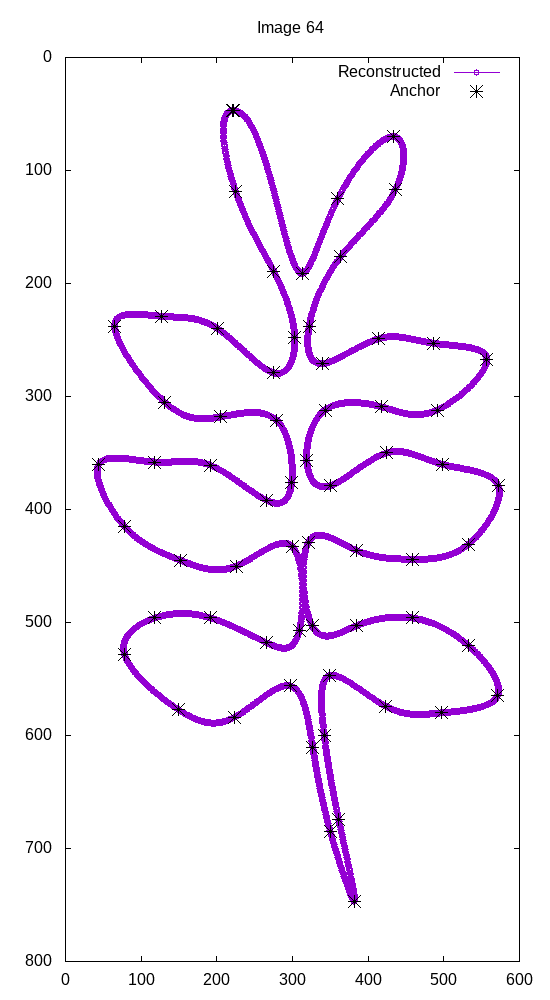
\includegraphics[width=\textwidth]{img/rec/64lin(24802).png}
			\caption{Linearmente espaçados (24802)}
		\end{subfigure}
		\begin{subfigure}[t]{0.24\textwidth}
			\centering
			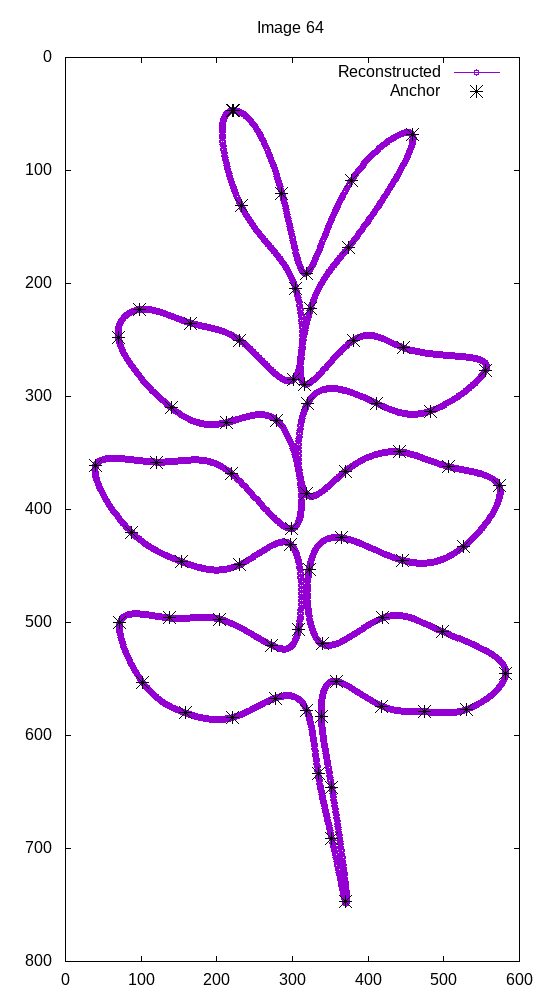
\includegraphics[width=\textwidth]{img/rec/64cur(26573).png}
			\caption{Curvatura (26573)}
		\end{subfigure}
		\begin{subfigure}[t]{0.24\textwidth}
			\centering
			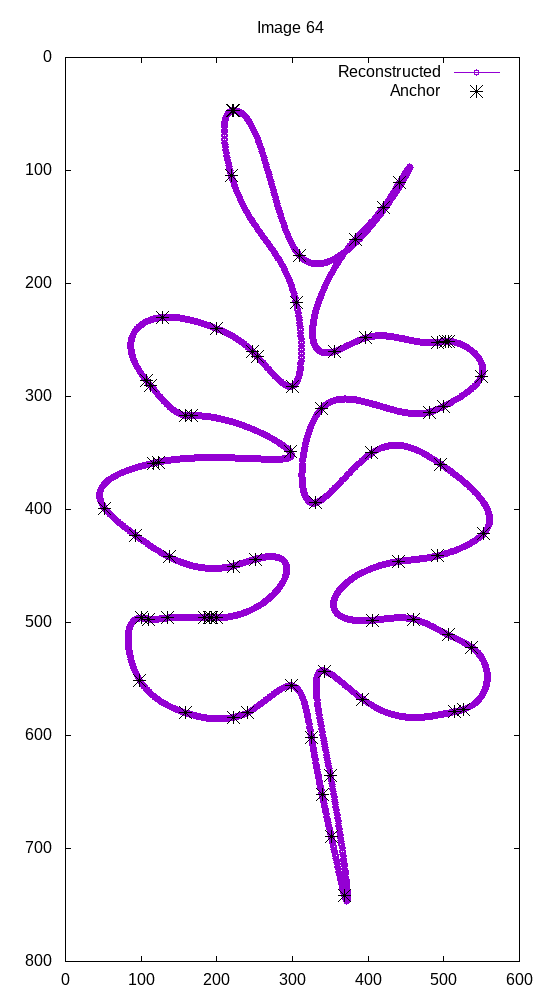
\includegraphics[width=\textwidth]{img/rec/64rng(50891).png}
			\caption{Aleatórios (50891)}
		\end{subfigure}
		\label{fig:rec6}
	\end{figure}
\end{frame}




\section{Problemas encontrados}
\begin{frame}
	\frametitle{Problemas encontrados}
	
	\begin{itemize}
		\item Alguns problemas com pré-processamento e extração de contorno com OpenCV;
		\item O método de Sorkine não funciona muito bem para figuras com muitas pontas (necessita de mais pontos âncora) - talvez isso não seja um problema para faces, mas será necessário testar.
	\end{itemize}
	
\end{frame}




\section{Próximos passos}
\begin{frame}
	\frametitle{Próximos passos}
	
	\begin{itemize}
		\item Corrigir parte de pré-processamento;
		\item Testar para casos mais gerais (incluindo curvas de faces no $\mathbb{R}^3$);
		\item Conferir melhores métricas para avaliar as curvas obtidas e outras técnicas de obter os pontos âncora.
	\end{itemize}
	
\end{frame}




%%%%%%%%%%%%%%%%%%%%%%%%%%%%
\section{Referências}

%\nocite{*}
\begin{frame}[allowframebreaks]
  \frametitle{Referência Bibliográfica}
  \bibliographystyle{siam}
  
  \bibliography{referencias}
\end{frame}

\end{document}
